\documentclass[10pt]{article}%
% \documentclass[nofootinbib,preprint,floatfix,endfloats]{revtex4} % ,endfloats,floatfix
%\documentclass[12pt,a4paper,final]{iopart}

\usepackage[utf8]{inputenc}
\usepackage{nima,graphicx,amsmath,amssymb,color}%,hyperref}
\usepackage{mathrsfs}
%\usepackage{graphicx}
\usepackage{comment}
\usepackage{setspace}
% \newcommand{\Ls}{\mathscr{L}}

% \newcommand{\lrto}{\leftrightarrow}
 \marginparwidth 0pt
 \oddsidemargin  0pt
 \evensidemargin  0pt
 \marginparsep 0pt
 \topmargin   -1.25in 
\textwidth   6.5in
 \textheight  10.0 in
\newcommand{\RNum}[1]{\uppercase\expandafter{\romannumeral #1\relax}}
\newcommand{\outNim}[1]{}
%

\begin{document}
\title{Phases of Physical 3D Networks}
\author{Nima Dehmamy\thanks{nidami@gmail.com}, Soodabeh Milanlouei, Albert-L\'aszl\'o Barab\'asi \\
{\em CCNR, Northeastern University, Boston, 02115 MA} }
% \date{\today}
\maketitle
% {
In networks, such as neurons connecting to form a brain, the nodes and links have physical reality, unable to overlap or cross each other. 
These non-crossing conditions and the tight-packed nature of nodes and links determine their physical layout and limit how these networks can form and evolve. 
These features cannot be captured by the current network layout models which ignore the physical dimensions of the links and nodes, assuming that they are largely invisible to each other. 
Here we explore the constraints the physical nature of the nodes and links impose on the layout of real networks. 
We do so by developing a 3D layout algorithm that observes the physical reality of the components, allowing us to systematically explore how these constraints affect the layout. 
For small link diameters, we observe a weakly interacting phase, where links bend locally to avoid crossings,but the network layout remaining largely unchanged, and the relative link diameter reaches a critical threshold, we observe a transition to a new strongly interactive phase, where the layout is fundamentally reorganized by the excluded volume interactions between the links. 
We determine the scaling of this transition point, and show that a whole host of topological quantities, from the total link weights to the relative angles of nearby links and link curvatures, undergo major changes at the transition point. 
We also find an amazing universality in each phase, the network layout being largely independent of the underlying network topology. 
Finally, we document systematic changes in the physical properties of the obtained networks, finding that in the strongly interacting phase the network responds to external pressure as a liquid, but developing solid-like properties in the weakly interacting phase. 
These findings not only determine the fundamental implicating of the constraints real physical networks need to obey, but also offer insights on the layout of mammalian brains, and have implications for the 3D printing of realistic networks.
% }

\begin{figure}[hb]
\caption{3D layouts  using ELM and E-ELM, and their phase diagram.}
    
    % \centering
    %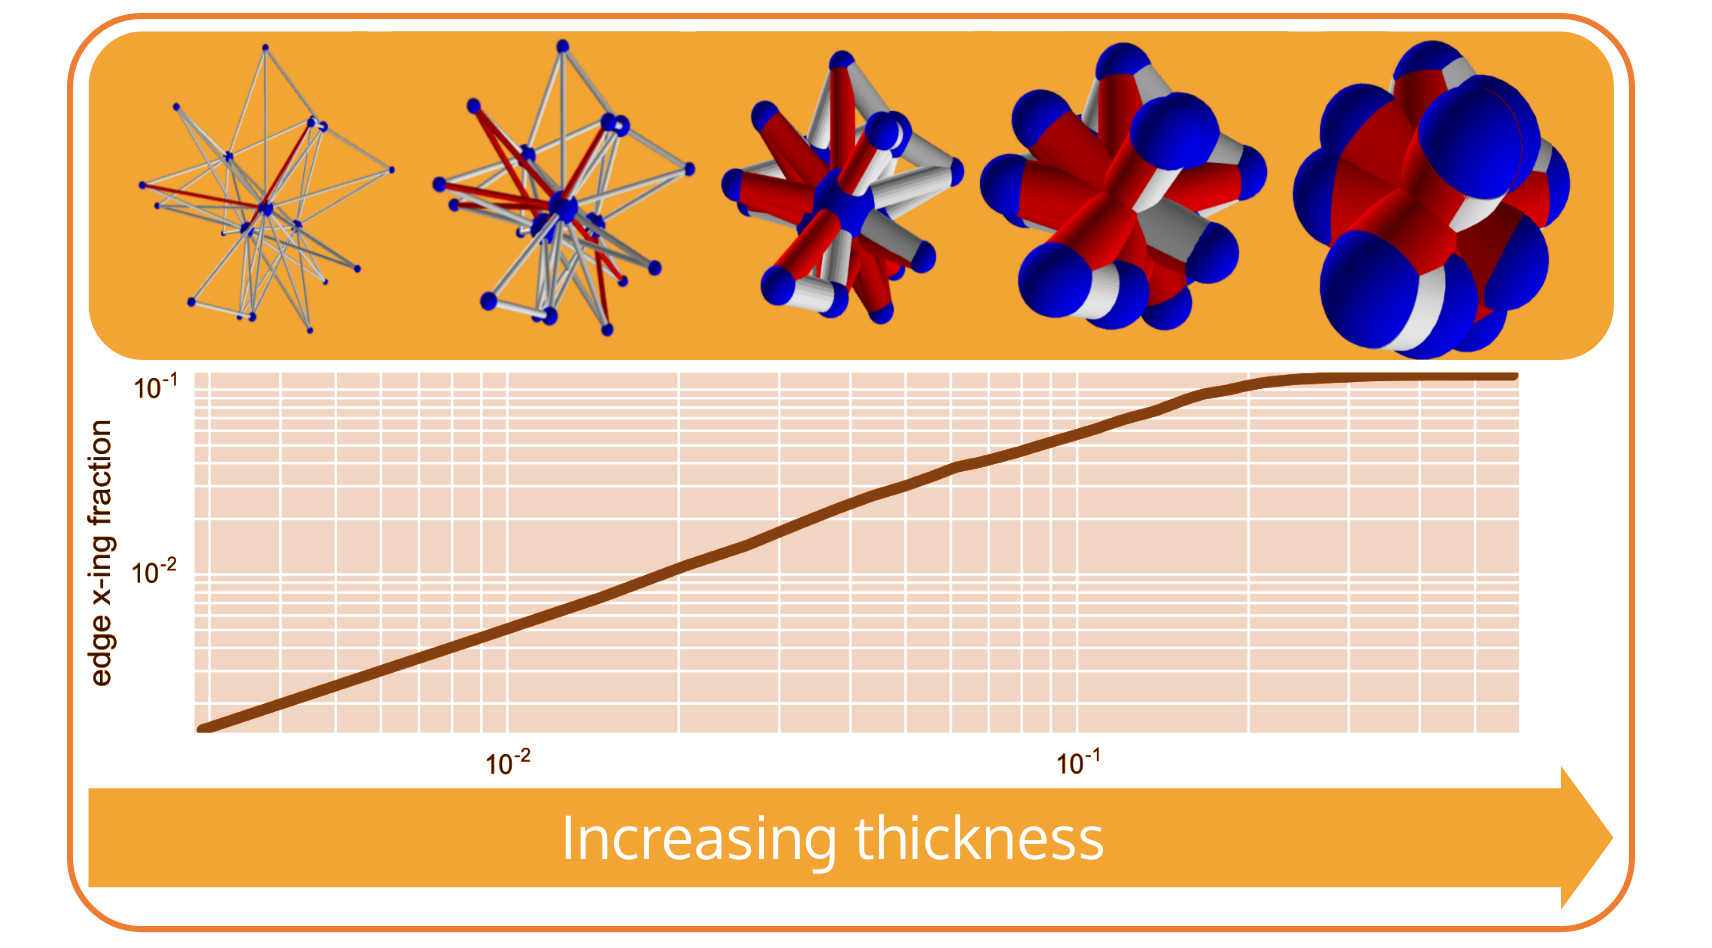
\includegraphics[width=.63\columnwidth]{fig-09-19/crs-panel.png}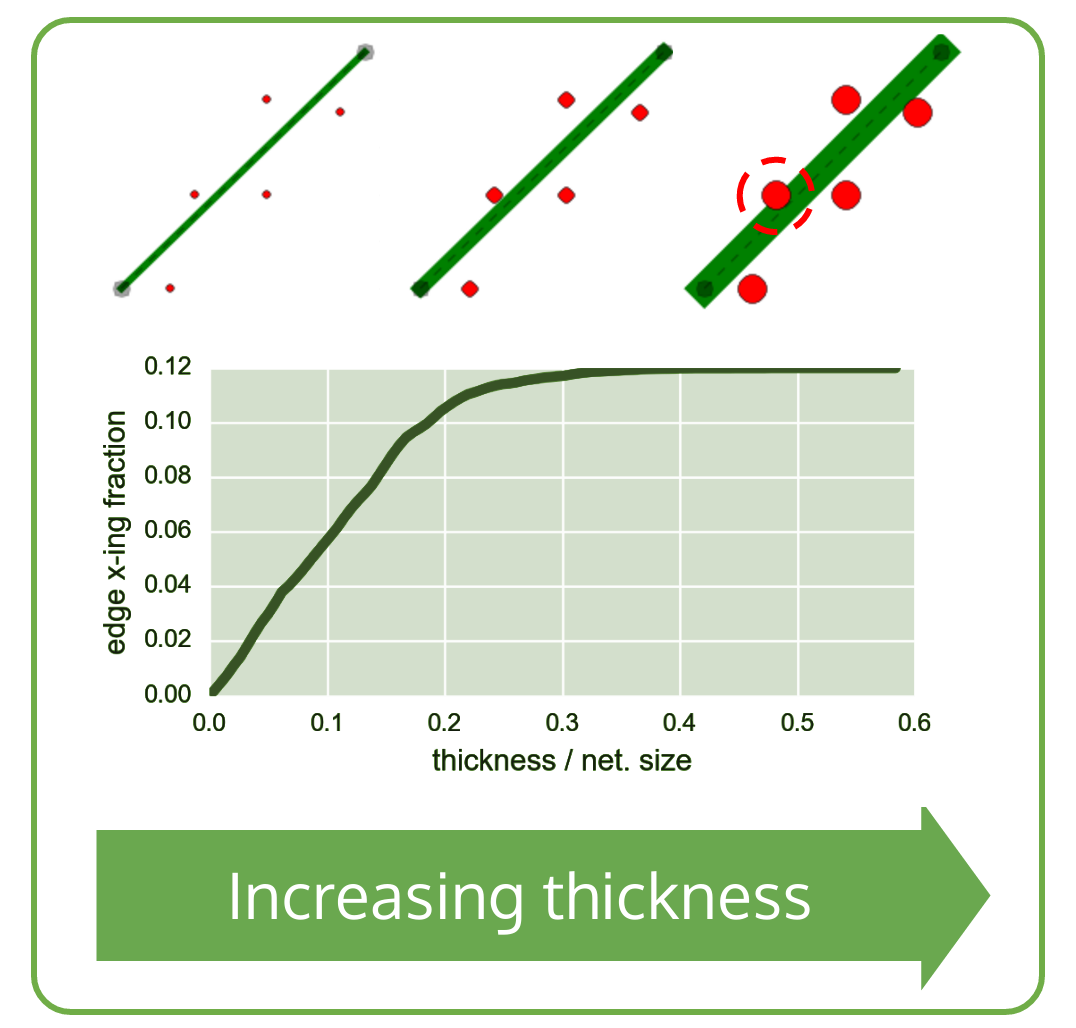
\includegraphics[width=.365\columnwidth]{fig-09-19/crs-2d-panel-green-2.png}
    \begin{tabular}{ll}
    \begin{minipage}{.7\columnwidth}
    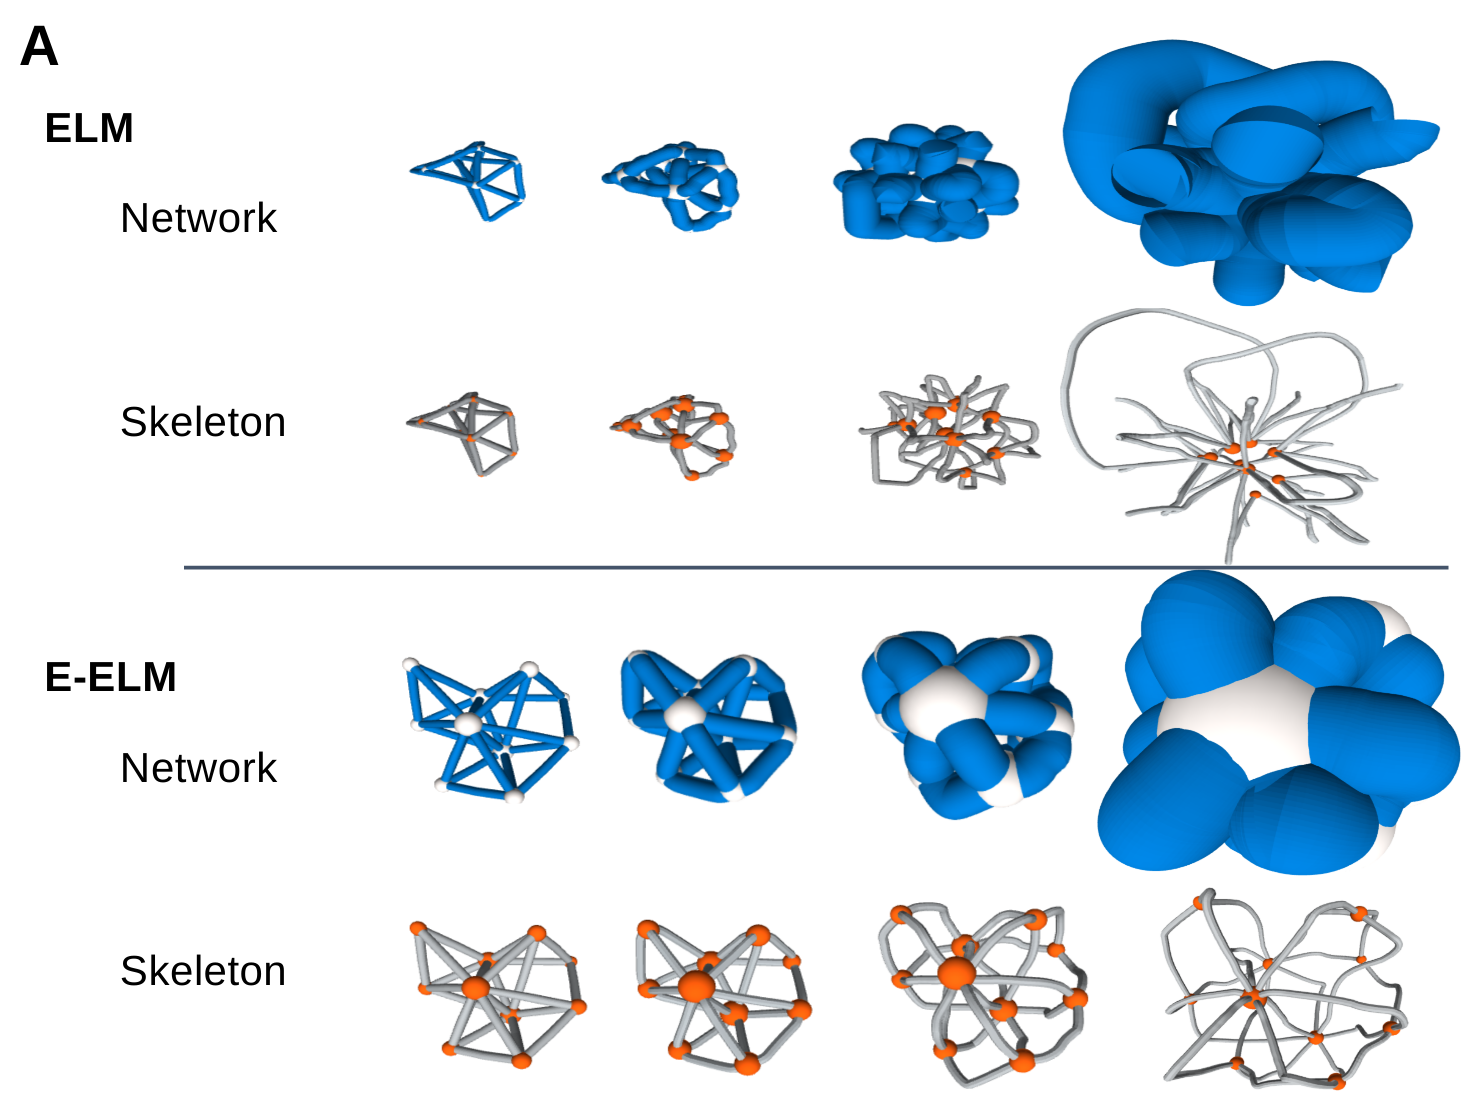
\includegraphics[width=\columnwidth]{fig-09-19/viz.png}
    \end{minipage}
         &
        %  \makebox[.3\columnwidth]{hi}
         \begin{minipage}{.3\textwidth}
         \raggedright
         \begin{spacing}{.5}
         {\scriptsize {\bf Our two layout algorithms, ELM and E-ELM, at various link thicknesses:} \\ ELM and E-ELM used on a BA $N=10, m=3$. Pictures with blue links are actual size. Gray links are thinned down to show the skeleton of the layout.  At small thicknesses, $r$, both layouts are the similar to FDL. At larger $r$ in ELM links start bending to avoid each other. At very large $r$, links don't fit inside the region containing the nodes and start making outward arcs. E-ELM at large $r$ behaves more gently and the layout size just grows linearly with the $r$.}
        \end{spacing}
    \end{minipage}\\
    % \hline
    % \begin{minipage}{.7\columnwidth}
    % 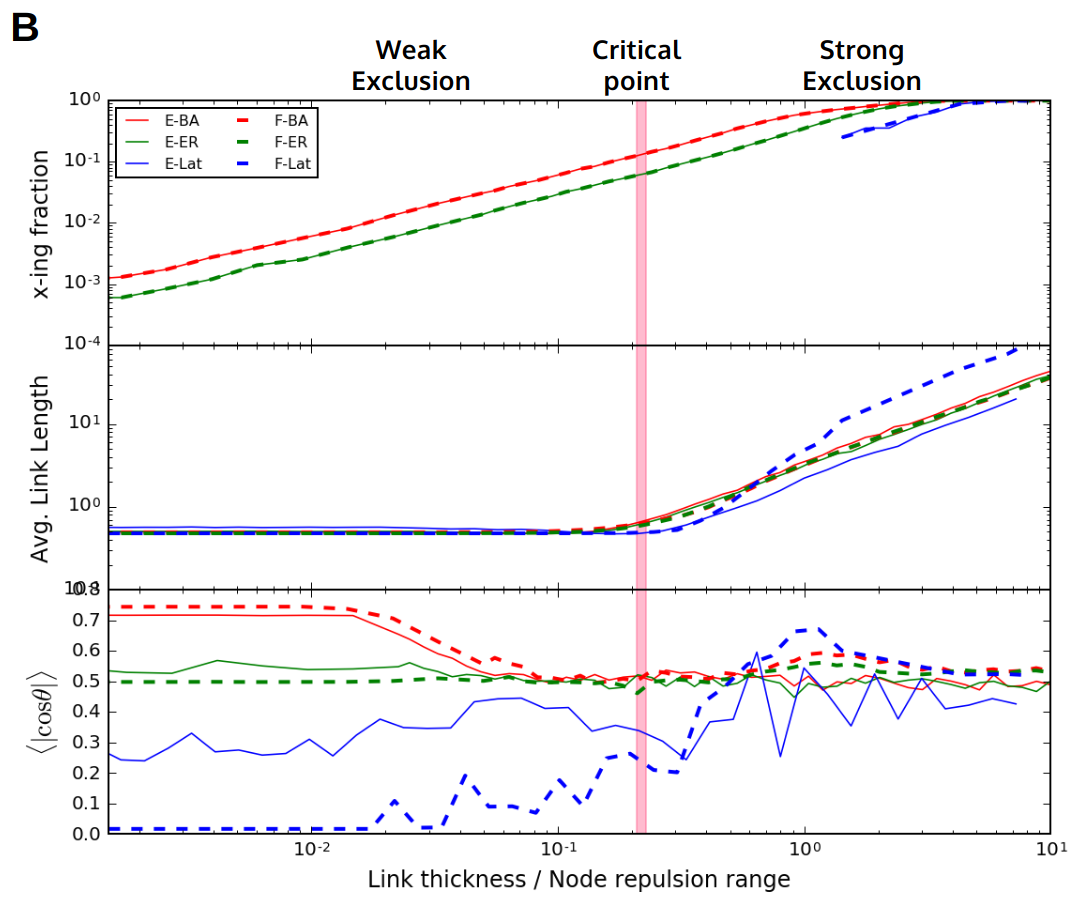
\includegraphics[width=\columnwidth]{fig-09-19/phase.png}
    % \end{minipage}
    % &
    % \begin{minipage}{.3\textwidth}
    %      \raggedright
         
    % \begin{spacing}{.5}
    % {\scriptsize
    % ~\\
    % \bigskip
    %      {\bf Phases of ELM vs. E-ELM:} 
    %      Fraction of crossing links, average link length, average relative angle of adjacent link segments $\be{|\cos\theta |}$, and total tensile stress in nodes and links. Dashed lines correspond to ELM (prefix ``F-'' in legend) and solid ones are E-ELM (prefix ``E-'') layouts. Each color signifies a network topology: ER: Erdős-Renyi; BA: Barabasi-Albert; Lat: the 3D regular lattice.  The average link length (second plot) and the total tensile stress build-up (fourth plot) are not good discriminants of different network topologies. Neither does it distinguish between ELM and E-ELM. The $\be{|\cos\theta |}$, on the other hand, does discriminate between both topology and the two layouts ELM and E-ELM in the  ``weak exclusion phase''. In the ``strong exclusion phase'' at large link thickness, however, different topologies laid out using ELM are indistinguishable. Same is true of the strong exclusion phase in E-ELM.
    % }
    % \end{spacing}
    % \end{minipage}
         
    \end{tabular}
    \label{fig:phase}
\end{figure}

\end{document}